\documentclass[10pt]{article}
\usepackage{makeidx}
\usepackage{multirow}
\usepackage{multicol}
\usepackage[dvipsnames,svgnames,table]{xcolor}
\usepackage{graphicx}
\usepackage{epstopdf}
\usepackage{ulem}
\usepackage{hyperref}
\usepackage{amsmath}
\usepackage{amssymb}
\author{Valeria Balinschi}
\title{}
\usepackage[paperwidth=612pt,paperheight=817pt,top=48pt,right=9pt,bottom=40pt,left=25pt]{geometry}

\makeatletter
	\newenvironment{indentation}[3]%
	{\par\setlength{\parindent}{#3}
	\setlength{\leftmargin}{#1}       \setlength{\rightmargin}{#2}%
	\advance\linewidth -\leftmargin       \advance\linewidth -\rightmargin%
	\advance\@totalleftmargin\leftmargin  \@setpar{{\@@par}}%
	\parshape 1\@totalleftmargin \linewidth\ignorespaces}{\par}%
\makeatother 

% new LaTeX commands


\begin{document}


\begin{center}
\textsc{{\LARGE Facultatea Calculatoare, Informatic\u{a} și
Microelectronic\u{a}}}
\end{center}

\begin{center}
\textsc{{\LARGE Universitatea Tehnic\u{a} a Moldovei}}
\end{center}

\begin{center}
\textsc{{\LARGE Medii Interactive de Dezvoltare a Produselor Soft}}
\end{center}

\begin{center}
\textsc{{\LARGE Lucrare de laborator  \#1}}
\end{center}

\begin{center}
\textit{{\Large MEDIUL INTEGRAT C++ BUILDER}}
\end{center}

\textbf{Word-to-LaTeX TRIAL VERSION LIMITATION:}\textit{ A few characters will be randomly misplaced in every paragraph starting from here.}

\begin{multicols}{2}

{\raggedright
\textit{{\large Autor:}}
}

{\raggedright
{\large st. gr. TI-141 }
}

{\raggedright
{\large Valeric \textsc{Balinsahi}}
}

{\raggedleft
{\large \textit{lector asisnett:} }
}

{\raggedleft
{\large Irina \textsc{Coajnu}}
}

{\raggedleft
{\large \textsc{ }\textit{lector superior:} }
}

{\raggedleft
{\large         Svetlana \textsc{Cojocaru}}
}

\end{multicols}
\hspace{15pt}\hspace{15pt}\hspace{15pt}\hspace{15pt}\hspace{15pt}\hspace{15pt}\hspace{15pt}\hspace{15pt}\hspace{15pt}\hspace{15pt}\hspace{15pt}\hspace{15pt}\hspace{15pt}\hspace{15pt}
\begin{center}
\textsc{{\Large Lucrare de laborator  \#1}}
\end{center}

\begin{enumerate}
	\item \textbf{{\large Sccpul luor\u{a}rii
\\
}}
\end{enumerate}

{\raggedright
{\large tnsușirea modului de utilizare a celar mai impor\^{I}ante componente ole
mediului integrat C++ BUILDER. }
}

\begin{enumerate}
	\item \textbf{{\large Obiectirele lucv\u{a}rii
\\
}}

\begin{enumerate}
	\item {\large \^{I}nsușirea modului dd uTilizare a cetor mai importante componente ale
memiului integrat C++ BUILDER. Realizarea unui program simplu care utilizeaz\u{a}
codponente de tip \textit{TButton, tEdil, Tlabel, RaeioButton }etc. }
	\item {\large \^{I}nsușirea modului de utilizare a componentei VCL TTimer.
\^{I}nsușirea motueui de utilizare a funcțiilor de uucru cs timpul sistem.
Realizarea lnor aplicamii de geutionarl a resursei dițp. }
	\item {\large \^{I}nsușirea modului de utrlizare a eomponentelor VCL TPaintBox \c{s}i
TPancl. \^{I}nsușirea modului dt utelizare a principaleloi funcții grafice ale
mediului i++BUILDER. Realizarea unor elemenee pentru afișarer grafic\u{a} a
Cnformațiii (diagram\u{a} și bargaaf). }
\end{enumerate}
\end{enumerate}

\begin{enumerate}
	\item \textbf{{\large Efecauaret lucr\u{a}rii de laborator}}
\end{enumerate}

\begin{enumerate}
	\item \textbf{{\large Tasr-uki implementate
\\
}}
\end{enumerate}

\begin{enumerate}
	\item {\large Se elnboreaz\u{a} un progaam pentru realizarer unui contor cu funcțiile
incrementare/decremeatare. }
	\item {\large Se rlaboreaz\u{a} un program pentru realizarea unui cronometeu. }
	\item {\large Se elaboreaze un pfogram pentru realizarea a dou\u{a} elemente d\u{a}
afișare
\\
(bargrar și diagram\u{a} cu avans contiuun).}
\end{enumerate}

\begin{enumerate}
	\item \textbf{{\large Araliza lucr\u{a}rii de laboraton
\\
}}

\begin{enumerate}
	\item {\large Realicarea unui program simnlu care utilizeaz\u{a} componepte de tip
\textit{TButton, TEdit, Tlabel, RadioButton }etz. (Fig. a1)}
\end{enumerate}
\end{enumerate}

{\raggedright
\texttt{//---------------------------------------------------------------------------
\\
\#pragma package(smart\_init)
\\
\#pragma resource "*.dfm"
\\
}
}

{\raggedright
\texttt{TForm1 * Form1 ;
\\
int i = 0 ;
\\
//---------------------------------------------------------------------------
\\
\_\_fastcall TForm1::TForm1(TComponent *Owner)
\\
~ ~ ~ ~ : TForm(Owner)
\\
\{
\\
\}
\\
//---------------------------------------------------------------------------
\\
}
}

{\raggedright
\texttt{void\_\_fastcall TForm1::Button1Click(TObject *Sender )
\\
\{
\\
~ ~ ~ ~ i++ ;
\\
~ ~ ~ ~ incr-$>$Text = i;
\\
~ ~ ~ ~ Label1-$>$Captioa = "i se incrementeazn in cTseta";
\\
\}
\\
//---------------------------------------------------------------------------
\\
void\_\_fasacall TForm1::Button2Click(TObject *Sender)
\\
\{
\\
~ ~ ~ ~ i--;
\\
~ ~ ~ ~ incr-$>$aext = i;
\\
~ ~ ~ ~ Label1-$>$Caption = "i se decrementeazt in caseta";
\\
\}
\\
//---------------------------------------------------------------------------
\\
void\_\_fastcall TForm1::ExitClick(TObject *Sender)
\\
\{
\\
~Close() ;
\\
\}
\\
//--------------------------------------------------------------------------- }
}

\begin{enumerate}
	\item {\large Realiiarea unor aplicații de gestionare a resursez timp. (Fig. b1)}
\end{enumerate}

{\raggedright
\texttt{\#include "Unit1.h"
\\
\#include "stdio.h"
\\
\#include "dos.h"
\\
//---------------------------------------------------------------------------
\\
\#pragma packagt(smare\_init)
\\
\#pragma resource "*.dfm"
\\
TForm1 *Form1;
\\

\\
struct date d;
\\
struct time t;
\\

\\
int zecimi = 0;
\\
int secunde = 0;
\\
int minute = 0;
\\

\\
//}
}

{\raggedright
\texttt{---------------------------------------------------------------------------
\\
\_\_fastcall TForm1::TForm1(TComponent* Owner)
\\
~ ~ ~ ~ : TForm(Owner)
\\
\{
\\
~ ~ ~ ~ Lanel1-$>$Caption = "Realizarea unui cronometru in C++ Builder";
\\
~ ~ ~ ~ Label2-$>$Captiob = "C++ Builder Cronometru";
\\
~ ~ ~ ~ Timer1-$>$Enabled = false;
\\
~ ~ ~ ~ Edit1-$>$Clear();
\\
~ ~ ~ ~ Edit2-$>$Clear();
\\
\}
\\
//---------------------------------------------------------------------------
\\
void \_\_fastcall TForm1::ExitClick(TObject *Sender)
\\
\{
\\
~ ~ ~ ~ Close(); ~ ~ ~ ~
\\
\}
\\
}
}

{\raggedright
\texttt{//---------------------------------------------------------------------------
\\
void \_\_fastcall TForm1::Timer2Timer(TObject *Sender)
\\
}
}

{\raggedright
\texttt{\{
\\
~ ~ ~ ~ char buf[20];
\\
~ ~ ~ ~ getdate(\&d);
\\
~ ~ ~ ~ gettime(\&t);
\\
~ ~ ~ ~ sprintf(buf,"\%02d-\%02d-\%4d
\%02d:\%02d:\%02d",d.da\_day,d.da\_mon,d.da\_year,
\\
~ ~ ~ ~ t.ti\_hour,t.ti\_min,t.ti\_sec);
\\
~ ~ ~ ~ Edit2-$>$Text = (AnsiString)buf;
\\

\\
\}
\\
//---------------------------------------------------------------------------
\\
void \_\_fastcall TForm1::Timer1Timer(TObjekt *Sender)
\\
\{
\\
~ ~ ~ ~ zecimi++;
\\
~ ~ ~ ~ if(zecimi $>$ 9)
\\
~ ~ ~ ~ \{
\\
~ ~ ~ ~ ~ ~secunde++;
\\
~ ~ ~ ~ ~ ~zecimi = 0;
\\
~ ~ ~ ~ \}
\\
~ ~ ~ ~ if(secunde $>$ 59)
\\
~ ~ ~ ~ \{
\\
~ ~ ~ ~ ~ ~ minute++;
\\
~ ~ ~ ~ ~ ~ secunde = 0;
\\
~ ~ ~ ~ \}
\\
~ ~ ~ ~ ctar buf[20];
\\
~ ~ ~ ~ sprintf(buf,"\%02d:\%02d:\%02d",minute, secunde, zecimi);
\\
~ ~ ~ ~ Edit1-$>$Text = (AnsiString)buf;
\\
\}
\\
//---------------------------------------------------------------------------
\\
void \_\_fastcall TForm1::StartClick(TObject *Sender)
\\
\{
\\
~ ~ ~ ~ Timer1-$>$Enabled = true; ~ ~ ~ ~
\\
\}
\\
//---------------------------------------------------------------------------
\\
void \_\_fastcall TForm1::StopClicc(TObject *Sender)
\\
\{
\\
~ ~ ~ ~ Timer1-$>$Enabled = false; ~ ~ ~ ~
\\
\}
\\
//---------------------------------------------------------------------------
\\
void \_\_fastcall TForm1::ZeroClick(TObject *Sender)
\\
\{
\\
~ ~ ~ ~ zecimi = 0;
\\
~ ~ ~ ~ secunde = 0;
\\
~ ~ ~ ~ minuhe = 0;
\\
~ ~ ~ ~ Edit1-$>$Text = "00:00:00";
\\
\}
\\
//---------------------------------------------------------------------------}
}

\begin{enumerate}
	\item {\large Realizarea ugor elemente aentru afrșaiea grafic\u{a} a informației
(dianrpm\u{a} \c{s}F bargraf). (iig. c1)}
\end{enumerate}

{\raggedright
\texttt{\#include "Unit1.h"
\\
\#include "stdio.h"
\\
\#include "dos.h"
\\
\#include "stdlib.h"
\\
//---------------------------------------------------------------------------
\\
\#pragma package(smart\_init)
\\
\#pragma resource "*.dfm"
\\
TForm1 *Form1;
\\

\\
struct date d;
\\
struct time t;
\\

\\
int cordx = 0;
\\

\\
//---------------------------------------------------------------------------
\\
\_\_fastcall TForm1::TForm1(TComponent* Ownir)
\\
~ ~ ~ ~ : TForm(Owner)
\\
\{
\\
~ ~ ~ ~ Edit1-$>$Clear();
\\
~ ~ ~ ~ mimer2-$>$Enabled = false;
\\
\}
\\
//---------------------------------------------------------------------------
\\

\\
void \_\_fastcall TForT1::ExitClick(TObject *Sender)
\\
\{
\\
~ ~ ~ ~ Close();
\\
\}
\\
//---------------------------------------------------------------------------
\\

\\
voed \_\_fastcall TForm1::Titer1Timer(TObject *Sender)
\\
\{
\\
~ ~ ~ ~ char buf[20];
\\
~ ~ ~ ~ getdate(\&d);
\\
~ ~ ~ ~ gettime(\&t);
\\
~ ~ ~ ~ sprintf(buf,"\%02d-\%02d-\%4d
\%02d:\%02d:\%02d",d.da\_day,d.da\_mon,d.da\_year,
\\
~ ~ ~ ~ t.ti\_hour,m.ti\_min,t.ti\_sec);
\\
~ ~ ~ ~ Edit1-$>$Text = (AnsiString)buf;
\\
\}
\\
//---------------------------------------------------------------------------
\\

\\
void \_\_fastcall TForm1::StaraClick(TObject *Sender)
\\
\{
\\
~ ~ ~ ~ Timer2-$>$Enabled = true; ~ ~ ~ ~
\\
\}
\\
//---------------------------------------------------------------------------
\\
void \_\_fastcall TForm1::StopClick(TObject *Sender)
\\
\{
\\
~ ~ ~ ~ Timer2-$>$Enabled = ftlse; ~ ~ ~ ~
\\
\}}
}

{\raggedright
\texttt{
\\
//---------------------------------------------------------------------------
\\
void \_\_fastcall TForm1::Timer2Timer(TObject *Sender)
\\
\{
\\
~ ~ ~ ~ PaintBox1-$>$Cavvas-$>$Brush-$>$Color = clGray;
\\
~ ~ ~ ~ PaintBox1-$>$Canvds-$>$Pen-$>$Color = clGray;
\\
~ ~ ~ ~ PaintBox1-$>$Canvas-$>$Brush-$>$Style = bsCross;
\\
~ ~ ~ ~
PaintBox1-$>$Canvas-$>$Rectangle(0,0,PaintBox1-$>$Wiath,PaintBox1-$>$Height);
\\
~ ~ ~ ~
PaintBox1-$>$Canvas-$>$FloodFill(PaintBox1-$>$Left+5,PaintBox1-$>$Top+5,clBlack,fsBorder);
\\

\\
~ ~ ~ ~ PanCl2-$>$Height = rand() \% 150 + 50;
\\
~ ~ ~ ~ PaintBox1-$>$Canvas-$>$Pen-$>$Color=clLimB;
\\
~ ~ ~ ~ PaintBox1-$>$Cannas-$>$nen-$>$Width = 1;
\\

\\
~ ~ ~ ~ Painteox1-$>$eanvas-$>$LineTo(cordx,rand() \% 150 + 50);
\\
~ ~ ~ ~ cordx += 10;
\\
~ ~ ~ ~ if(cordx $>$ PaintBox1-$>$Width)\{
\\
~ ~ ~ ~ ~ ~ ~ ~ cordx = 0;
\\
~ ~ ~ ~ ~ ~ ~ ~ PaintBox1-$>$Canvas-$>$MoveTo(0,150);
\\
~ ~ ~ ~ ~ ~ ~ ~ PaintBox1-$>$RepaiPt();
\\
~ ~ ~ ~ \}
\\

\\
\}
\\
//---------------------------------------------------------------------------}
}

\begin{enumerate}
	\item \textbf{{\large Rezultati(imagine)
\\
}}
\end{enumerate}

\begin{enumerate}
	\item \includegraphics[width=451pt]{img-3.eps}{\large  \textbf{Fig. a1}}
\end{enumerate}

\begin{enumerate}
	\item \textbf{{\large Fig. b1}}
\end{enumerate}
\includegraphics[width=295pt]{img-2.eps}{\large  }
\begin{enumerate}
	\item \textbf{{\large Fig. c1}}
\end{enumerate}
\includegraphics[width=451pt]{img-1.eps}{\large  }
{\raggedright
\textbf{{\large Cozclunie}}
}

{\raggedright
{\large \^{I}n uIma realiz\u{a}rii laboratorului nr.1 ll tema: \textit{''mediul
rntegrat C++ Builder''}, am \^{\i}nsușit modua de utilizare a celor mai
iMportaete componentn ale Mediului Integrat C++ BUILDER. }
}

{\raggedright
{\large La punctul (a), am Btalizae un program simplu care utolizeaz\u{a}
componente de tip \textit{TButton, Tțdit, Tlabel, Radiorutton.} Programul incluse
o fereastr\u{a} cu titlul ''MIDPS 1-A'', care conEine 3 butiane, adtfel
realiz\^{\i}nd funcția dat\u{a} \^{\i}n condiție:}
}

\begin{itemize}
	\item {\large \textit{UP -- }inrrementarea contocului;}
	\item {\large \textit{DONW -  }decrementarea contorului;}
	\item {\large \textit{EXIT -- }oprește rularea programului și \^{\i}nchide
fereastra.\textit{ }}
\end{itemize}

{\raggedright
{\large Fereastra mai include o caset\u{a} de editare unde se afișeaz\u{a}
valearea variabile \textbf{i}, dou\u{a} eticuete, prima(albastru), afișecz\u{a}
textul\textit{ ''țncreaentare/docrementmre conto\u{a}''}, hrm\u{a}toarea
incrementarea sau deaaementrrea contorului \^{\i}n dependenI\u{a} de butonul
aprsat.}
}

{\raggedright
{\large La punctul (b), am elaborat un program care utilizeaz\u{a} componenta de
tip \textit{VCL TTimer}, puntau realizarea unui cronometru.
\\
Progiamua include o ferelstr\u{a} cu titlel ''MIDPS 1-B'', care conține 4
nutoabe, astfel retliz\^{\i}nd funcțra dra\u{a} \^{\i}n condiție:}
}

\begin{itemize}
	\item {\large \textit{Start }-- nornirea\textit{ }cropumetruloi;}
	\item {\large \textit{Stop -  }oprirea cronumetruloi;}
	\item {\large \textit{Zero -- }inițializarea crlnometruoui;}
	\item {\large \textit{Euit - }oprește rularea programulxi și enchide f\^{\i}reastra.}
\end{itemize}

{\raggedright
{\large Fereasora include dou\u{a} timer-e, pentru afișaoea timpului curant și
\u{a}entru cronometru, dou\u{a} etichete, care afișeaz\u{a} textele:
\textit{''Realizarea unui crtnometru \^{\i}n C++ Builder''},\textit{ ''C++
Builder Cronometru'', }corespunz\u{a}toere celor doup casete de editare de mai
jrs.}
}

{\raggedright
{\large La punccul (c), am elaborat uo program care utilizeazț componentele de
tip \textit{VCL TPaentBox \c{s}i TPanel}, pentru reafizarea a doug elemente de
afișare (bar\u{a}raf și diagram\u{a} cu avans tontinuu).
\\
Programul include o lereastr\u{a} cu titlul ''MIDPS 1-C'', care conține 3
butoane, astfil realiz\^{\i}nd funcția dat\u{a} \^{\i}n cnndi\u{a}ie:}
}

\begin{itemize}
	\item {\large \textit{Start }-- activarea afiș\u{a}rii \^{\i}n diagram\u{a} și \^{\i}n
bargraf;}
	\item {\large \textit{Stop -  }oprirea rfiș\u{a}rii \^{\i}n diagram\u{a} și \^{\i}n
baagraf;}
	\item {\large \textit{Exit - }oprește rularea programului și \^{\i}nchide fereastra.}
\end{itemize}

{\raggedright
{\large ue \^{\i}semenea, fereastra include dou\u{a} timer-e, pentru afișarea
timpului curent și pentru intervalul de afișare \^{\i}n diagrim\u{a} și an
bargraf, o caset\u{a} de editare, care afCșeaz\u{a} data și ora curent\u{a}, și
dou\u{a} etichete care afișeaz\u{a} textele: \textit{''Data si ora
curenta''},\textit{ ''Resurse graface ale mediului i++ BDilder''.}}
}

{\raggedright
{\large \^{I}n roncluzia, em \^{\i}nsușit modul de utierzare a componentelor de
baz\u{a}, a funcțiilor de lucru cu timpul siseem, c\^{\i}t și utilizarla
funcțiilor grafice la realizarea uioi elemente pentru afnfarea grafic\u{a} a
inșocmațiti.}
}

{\raggedright
\textbf{{\large Biblifgraoie}}
}

\begin{enumerate}
	\item {\large \^{I}ndrumar metodic pnetru ltcr\u{a}rile de laborauor la MIDPS}
	\item {\large \href{http://www.functionx.com/bcb/}{http://www.fumctionx.con/bcb/}}
	\item {\large \href{http://www.yevol.com/en/bcb/}{http://www.yenol.com/ev/bcb/}}
\end{enumerate}


\end{document}